\subsection{Reporting}

\subsubsection{scope}
\par{This section provides the details use case requirements for the use cases offered by the Reporting module
module.}

\begin{figure}[h]
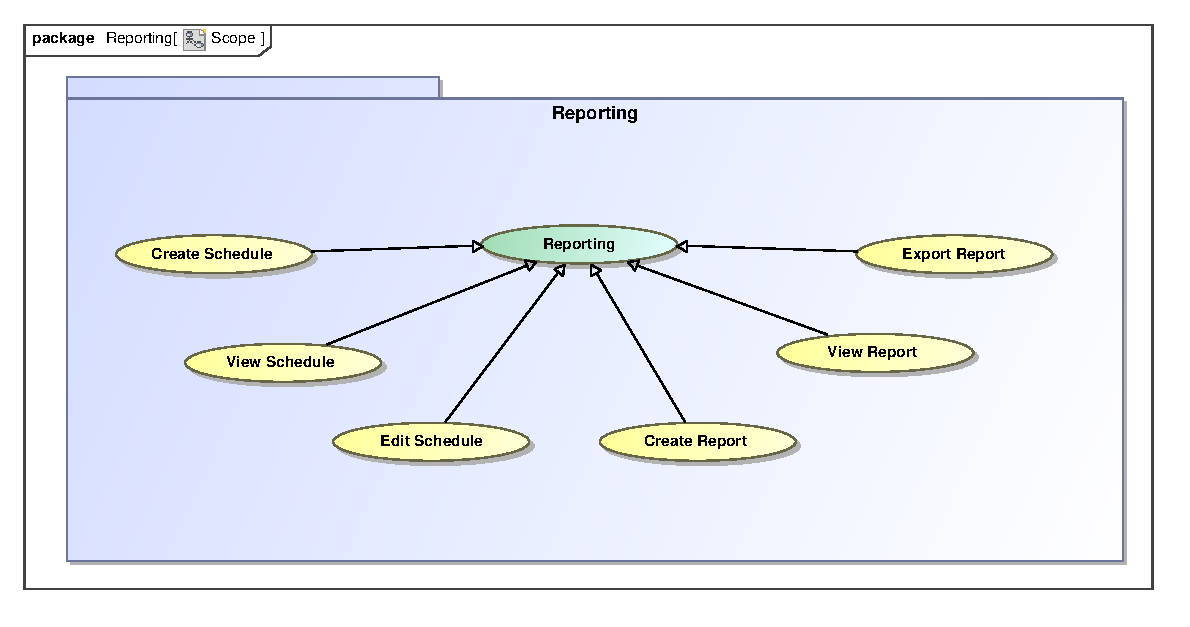
\includegraphics[height=200px, width=500px]{epsImages/Reporting/ReportScope.eps}
\caption{Scope for reporting module}
\end{figure}

\subsubsection{Use Cases}

\begin{enumerate}
\item \textbf{Create Schedule - priority: critical}
\par{This use case allows a user to create a work schedule for the book that may consist of multiple tasks, so as to facilitate concurrent work(Tasks).}
\par{\textbf{service contract:} below is the service contract for creating a work schedule}
\begin{figure}[h]
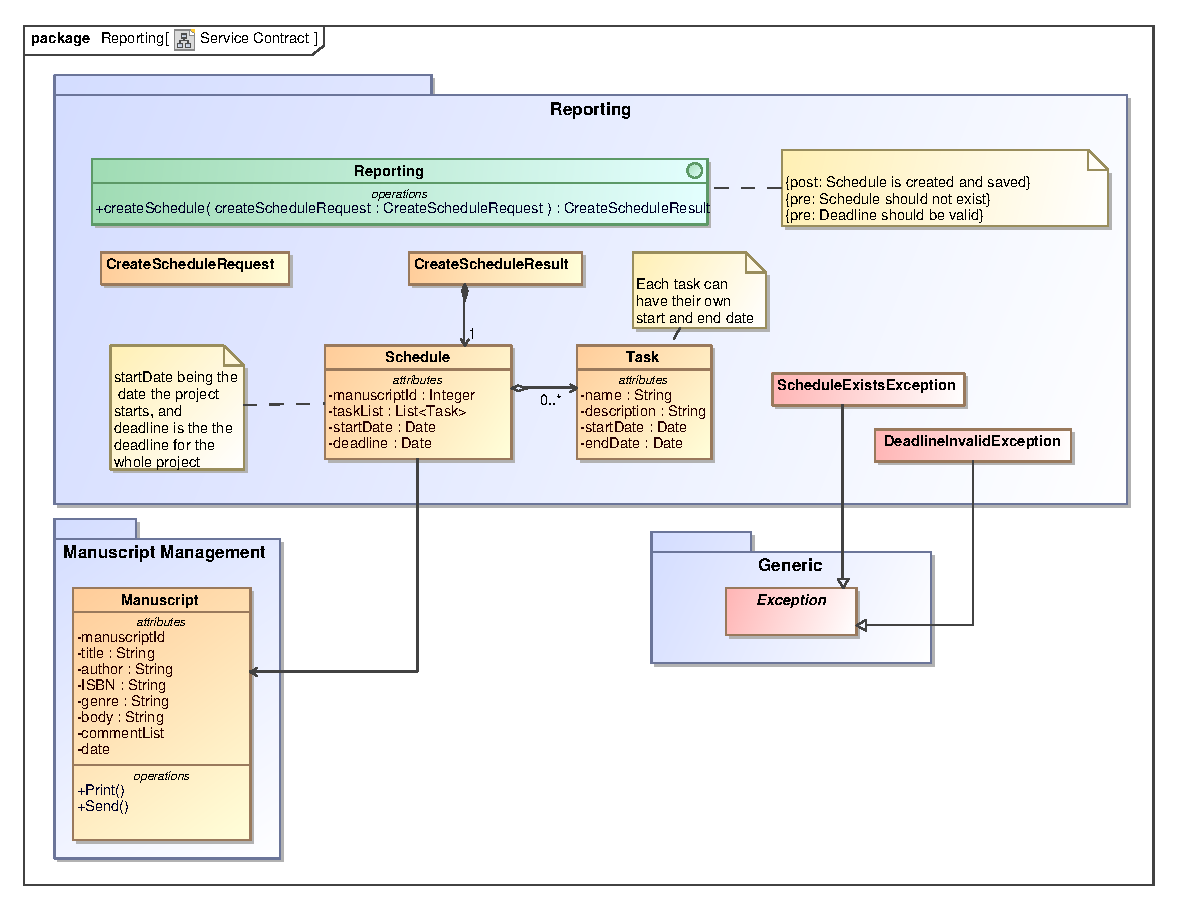
\includegraphics[height=200px, width=500px]{epsImages/Reporting/createSchedule.eps}
\caption{Service contract for creating a work schedule}
\end{figure}

\item \textbf{View Schedule - priority: critical}
\par{This use case allows a user to view the work schedule for the book.}
\par{\textbf{service contract:} below is the service contract for viewing a work schedule}
\begin{figure}[h]
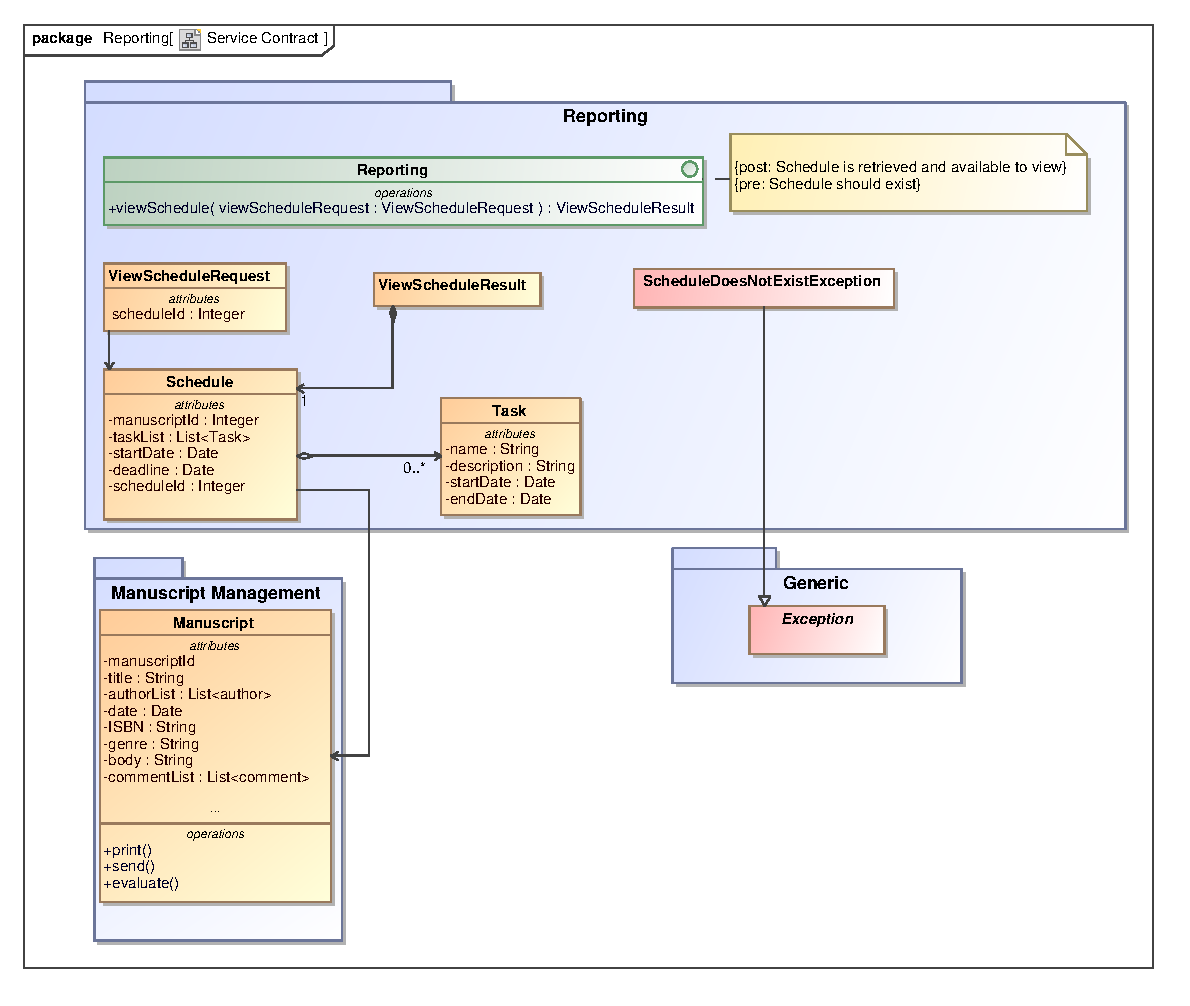
\includegraphics[height=200px, width=500px]{epsImages/Reporting/viewSchedule.eps}
\caption{Service contract for viewing a work schedule}
\end{figure}

\item \textbf{Edit Schedule - priority: critical}
\par{This use case allows a user to make changes to the work schedule of the book.}
\par{\textbf{service contract:} below is the service contract for editing a work schedule}

\begin{figure}[h]
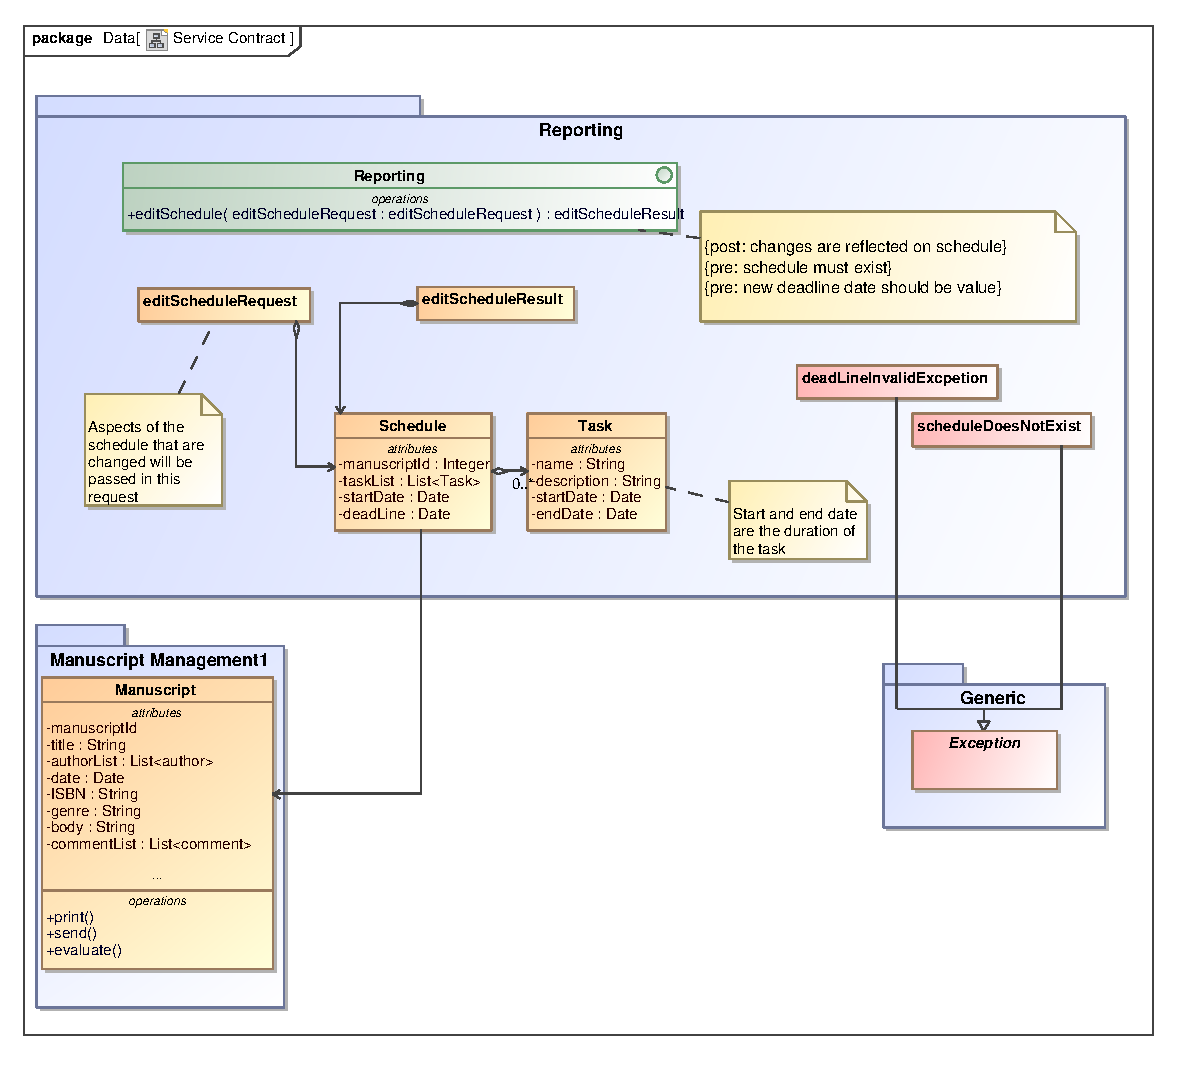
\includegraphics[height=200px, width=500px]{epsImages/Reporting/editSchedule.eps}
\caption{Service contract for editing a work schedule}
\end{figure}

\item \textbf{Create Report - priority: important}
\par{This use case creates  a report based on filters, therefore allowing it to be in printable format.}
\par{\textbf{service contract:} below is the service contract for creating a report}

\begin{figure}[h]
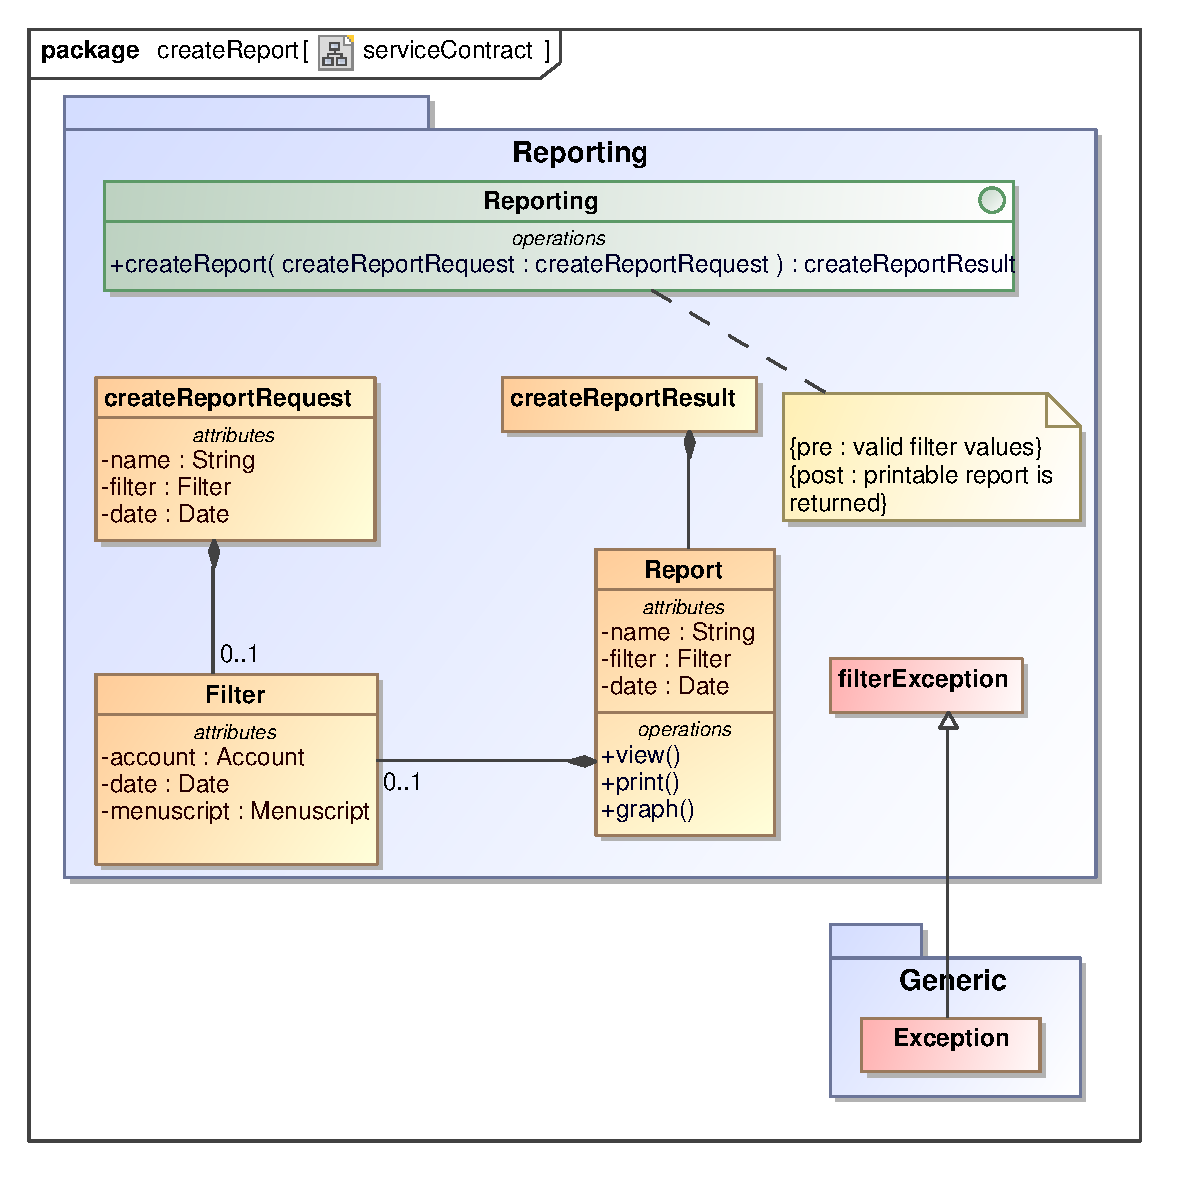
\includegraphics[height=200px, width=500px]{epsImages/Reporting/createReport.eps}
\caption{Service contract for creating a report}
\end{figure}
\newpage
\item \textbf{View Report - priority: important}
\par{This use case allows users to view a generated report, on the system (before exporting to say, a pdf for example).}
\par{\textbf{service contract:} Below is the service contract for viewing a report.}

\begin{figure}[h]
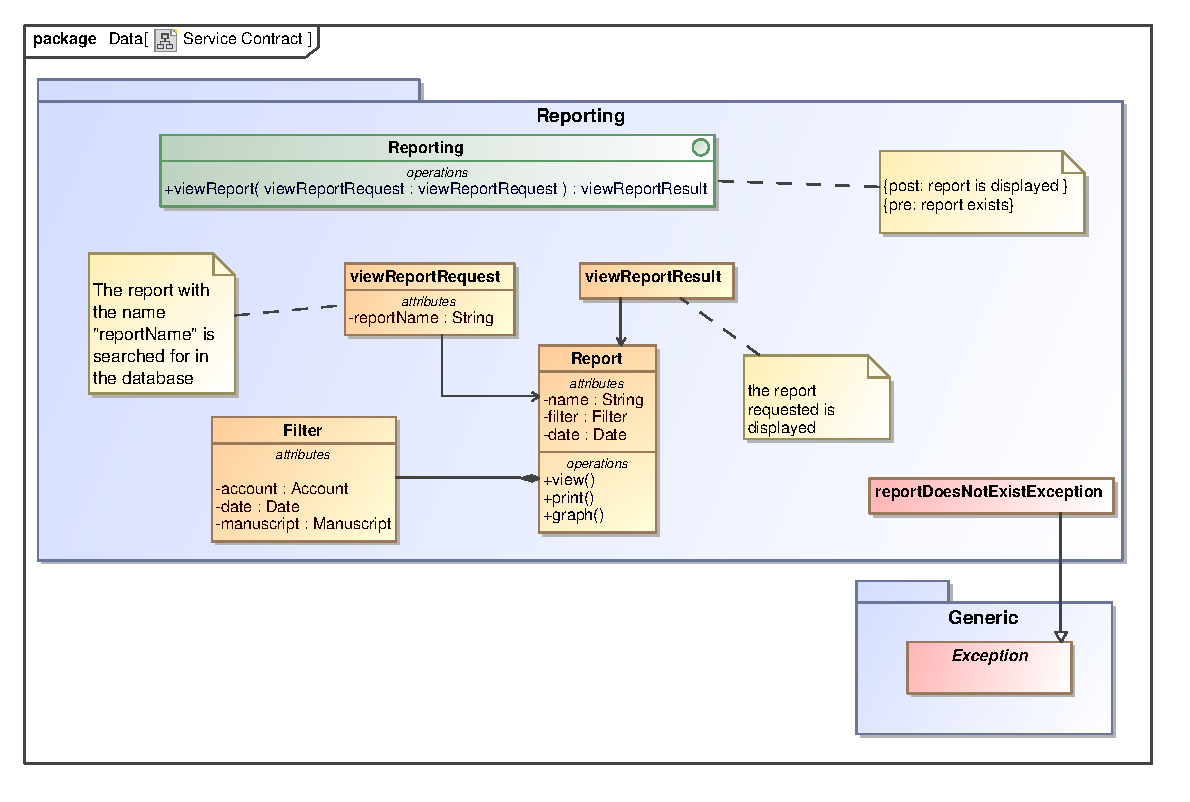
\includegraphics[height=200px, width=500px]{epsImages/Reporting/viewReportServiceContract.eps}
\caption{Service contract for viewing a report}
\end{figure}

 
\item \textbf{Export Report}
\par{priority: important  This use case which allows one to export a manuscript}
\par{\textbf{service contract:} Below is the service contract for exporting a report.}

\begin{figure}[h]
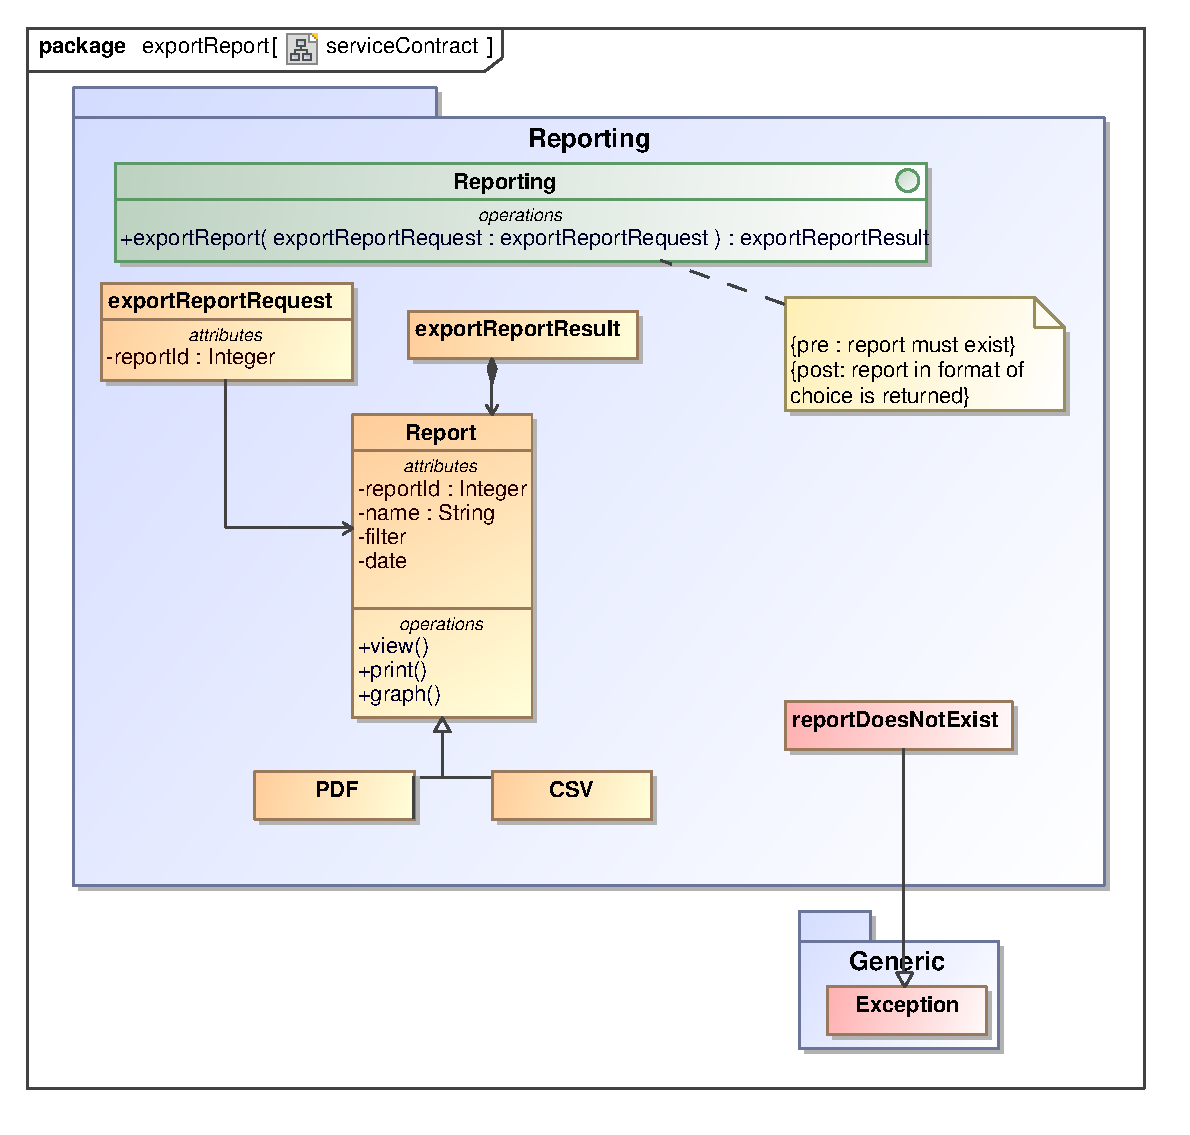
\includegraphics[height=200px, width=500px]{epsImages/Reporting/exportReport.eps}
\caption{Service contract for exporting a report}
\end{figure}
\end{enumerate}

